\chapter{Proposed Solution}\label{ch:solution}
Proposed solution goes here\dots

\section{Input Format}
\begin{itemize}
    \item Luma component (Y') of Y'UV representation
    \item Gradient magnitude of Sobel operator of luma component
    \item Canny edge map of luma component
    \item gPb
\end{itemize}

\section{Feature Extraction}
\begin{itemize}
    \item Global features: mean and standard deviation
    \item Local features: visual words via k-means clustering
\end{itemize}

\section{Distance Metric}
\begin{itemize}
    \item Euclidean Distance
\end{itemize}

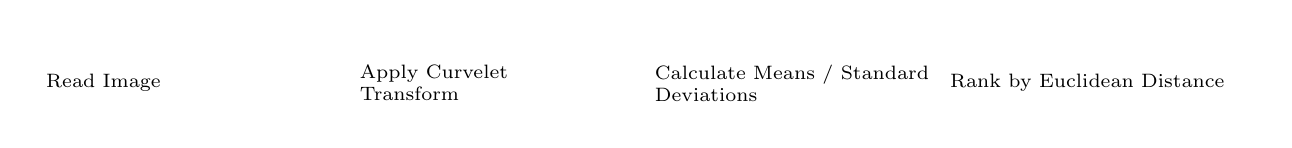
\begin{tikzpicture}[
        font=\scriptsize,
        point/.style={},
        block/.style={text width=10em}
    ]
    \matrix (thebigpicture) {
        % header
        \node[point] (colheader0) {}; &
        \node[point] (colheader1) {}; &
        \node[point] (colheader2) {}; &
        \node[point] (colheader3) {}; &
        \node[point] (colheader4) {}; &
        \node[point] (colheader5) {}; \\
        % first row
        \node[block] {Read Image}; & &
        \node[block] {Apply Curvelet \\ Transform}; &
        \node[block] {Calculate Means / Standard Deviations}; &
        \node[block] {Rank by Euclidean Distance}; \\
        \\
    };
\end{tikzpicture}
